\chapter{Planejamento do Sistema}

O planejamento do sistema é crucial para o sucesso do projeto. Nele deve-se estipular cronogramas de desenvolvimento e fazer a análise de risco para calcular a probabilidade e impacto de problemas que possam ocorrer durante o desenvolvimento do projeto.
Um bom planejamento também deve ter uma análise de projeto que envolva recursos de diversas naturezas bem como humanos, capitais, técnicos e tecnológicos.
Outro ponto importante é a prototipação do sistema para ter uma avaliação inicial com os \textit{stakeholders} e ter uma base a ser seguida durante o desenvolvimento.

\section{Cronograma do Projeto}

Todo bom projeto deve ter um cronograma e um planejamento de ação, baseado nisso, foi elaborado dois cronogramas: um apresentando todo o conteúdo aprendido no semestre e outro montando plano de ação para implementação do projeto.

As figuras a seguir, são cronogramas que demonstram a trajetória do desenvolvimento do projeto. Divididos por semestre, os cronogramas listam as atividades aprendidas nas UCs, com todas as partes teóricas e práticas onde o objetivo principal é implementar todo conhecimento adquirido em prol de um projeto único: A unificação de todas as UCs do curso de Sistemas para Internet.

\begin{figure}[H]
\caption{\label{cron-3-semestre}Cronograma de Aprendizagem: Terceiro Semestre}
\begin{center}
	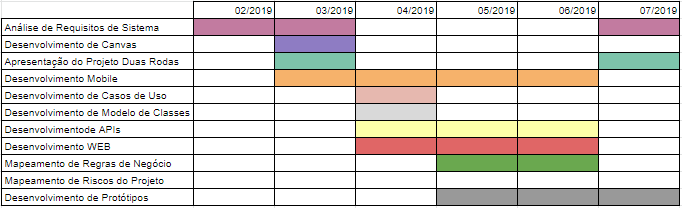
\includegraphics[scale=0.90]{./Figuras/cronograma-3-semestre.png}
\end{center}
\end{figure}


\begin{figure}[H]
\caption{\label{cron-4-semestre}Cronograma de Aprendizagem: Quarto Semestre}
\begin{center}
	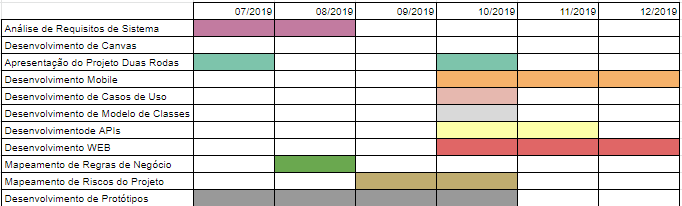
\includegraphics[scale=0.90]{./Figuras/cronograma-4-semestre.png}
\end{center}
\end{figure}


\begin{figure}[H]
\caption{\label{cron-5-semestre}Cronograma de Aprendizagem: Quinto Semestre}
\begin{center}
	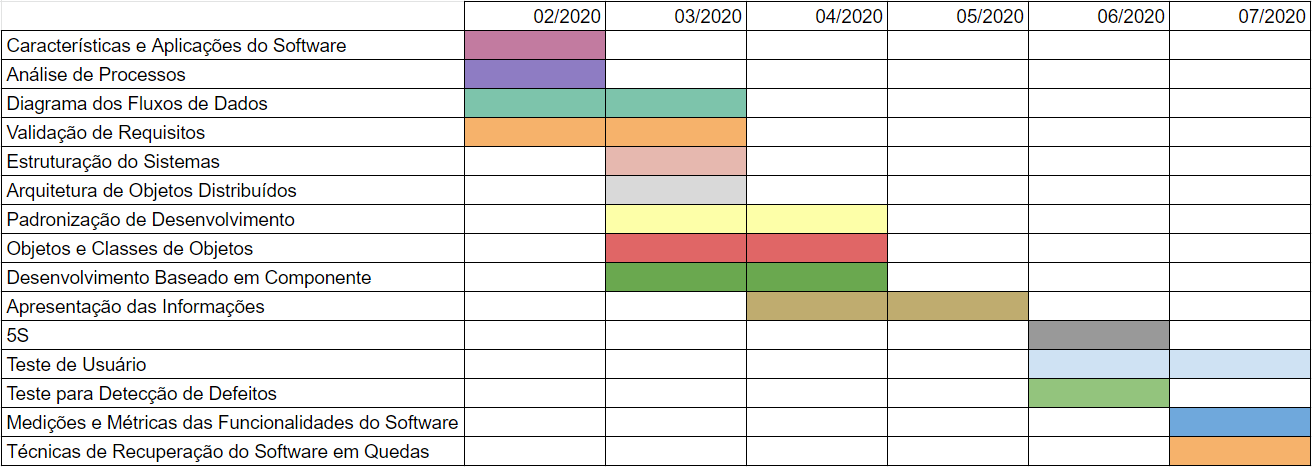
\includegraphics[scale=0.47]{./Figuras/cronograma-5-semestre.png}
\end{center}
\end{figure}

\begin{figure}[H]
	\caption{\label{cron-6-semestre}Cronograma de Aprendizagem: Sexto Semestre}
	\begin{center}
		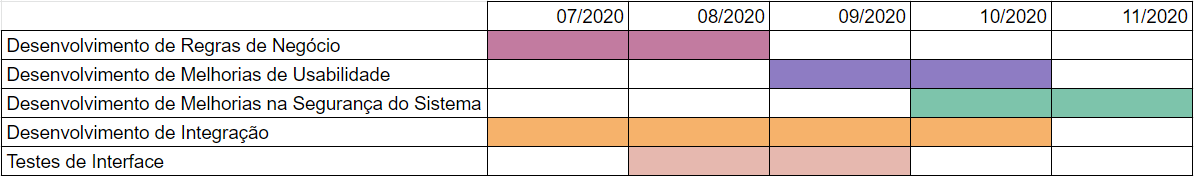
\includegraphics[scale=0.52]{./Figuras/cronograma-6-semestre.png}
	\end{center}
\end{figure}

\section{Análise de riscos}

A análise de riscos tem como objetivo identificar os possíveis problemas durante e após o desenvolvimento do projeto de modo a elaborar um plano de ação para solucionar rapidamente o problema de fato \cite{schmitzanalise}.

Segundo \cite{de2003engenharia}, um grande volume de dados publicados aponta para os riscos que correm os projetos de software executados sem a utilização de processos adequados. Um levantamento publicado, a partir de uma base de dados de 4000 projetos, constatou a ocorrência frequente dos seguintes problemas:

\begin{itemize}
	
	\item 70\% dos projetos de grandes aplicativos sofre de instabilidade dos requisitos. Os requisitos crescem tipicamente cerca de 1\% ao mês, atingindo níveis de mais de 25\% de inchaço ao final
	do projeto.
	
	\item Pelo menos 50\% dos projetos são executados com níveis de produtividade abaixo do normal.
	
	\item Pelo menos 25\% do software de prateleira e 50\% dos produtos feitos por encomenda apresentam níveis de defeitos superiores ao razoável. 
	
	\item Produtos feitos sob pressão de prazos podem quadruplicar o número de defeitos.
	
	\item Pelo menos 50\% dos grandes projetos de software estouram seu orçamento e seu prazo.
	
\end{itemize}

Sendo assim, foi identificado os fatores de risco, no qual o projeto em questão possa estar exposto. Nela, faz-se uma análise do impacto e probabilidade de fatores prejudiciais ao projeto, conforme tabela \ref{tebela_risco} abaixo.

\begin{table}[h]
	\centering
	\caption{\label{tebela_risco} Tabela de Riscos Agil.it}
	\begin{tabular}{l|l|l}
		\hline
		\rowcolor[HTML]{EFEFEF} 
		\textbf{Riscos}                     & \textbf{Probabilidade} & \textbf{Impacto} \\ \hline
		\rowcolor[HTML]{DD7346} 
		Mudança de escopo                   & 90\%                   & 2                \\ \hline
		\rowcolor[HTML]{DD7346} 
		Entrega no prazo                    & 70\%                   & 3                \\ \hline
		\rowcolor[HTML]{DD7346} 
		Integração com SAP                  & 70\%                   & 2                \\ \hline
		\rowcolor[HTML]{FFFE65} 
		Implantação na empresa              & 60\%                   & 2                \\ \hline
		\rowcolor[HTML]{FFFE65} 
		Conexão com o banco de dados        & 60\%                   & 3                \\ \hline
		\rowcolor[HTML]{FFFE65} 
		Aceitação da usabilidade do sistema & 50\%                   & 2                \\ \hline
		\rowcolor[HTML]{FFFE65} 
		Usuários inexperientes              & 40\%                   & 2                \\ \hline
		\rowcolor[HTML]{9AFF99} 
		Mudanças na tecnologia              & 20\%                   & 3                \\ \hline
		\rowcolor[HTML]{9AFF99} 
		Segurança dos dados                 & 15\%                   & 2                \\ \hline
		\rowcolor[HTML]{9AFF99} 
		Conexão com a rede                  & 10\%                   & 2                \\ \hline
		\rowcolor[HTML]{9AFF99} 
		Falta de profissionais              & 5\%                    & 3                \\ \hline
	\end{tabular}
	\legend{Fonte: os autores (2020)}
\end{table}

Na tabela \ref{tebela_risco} estão mapeados os principais riscos identificados para o projeto Agil.It. Nela, a probabilidade indica a chance do risco ocorrer, as cores acompanham a porcentagem da mesma, sendo 70\% ou mais a cor vermelha, entre 40\% e 69\% a cor amarela e de 0\% a 39\% a cor verde e o impacto é uma escala de um a três (1-3) do quanto o risco pode afetar a conclusão e entrega do projeto. A seguir será abordado o diagrama de causa e efeito.

\subsection{Diagrama de Causa e Efeito}

O diagrama de Ishikawa, diagrama espinha de peixe ou diagrama de causa e efeito foi desenvolvido por Kaoru Ishikawa em 1943 e é definida como uma representação gráfica usada como análise das causas de um determinado problema \cite{santos2017planos}.
O diagrama foi desenvolvido para consolidar os estudados realizados por uma fábrica e identificar as causas que deram início a ocorrência de um problema, por possibilitar a geração de melhorias e conhecimento do processo, os gestores utilizam amplamente \cite{ribeiro2017definiccao}.

Com a forma de uma espinha de peixe, o modelo original sugeria quatro grandes grupos de causas que deveriam ser analisadas. Esses quatro grupos (também conhecidos como quatro M's) eram: materiais, mão de obra, métodos e máquinas. Versões mais recentes desse diagrama sugerem a análise orientada por seis grandes grupos de causas: materiais, mão de obra, métodos, máquinas, medidas e meio ambiente \cite{selner1999analise}.

\begin{landscape}
	\begin{figure}[htb]
		\caption{\label{causaeefeito1}Diagrama de Causa e Efeito}
		\begin{center}
			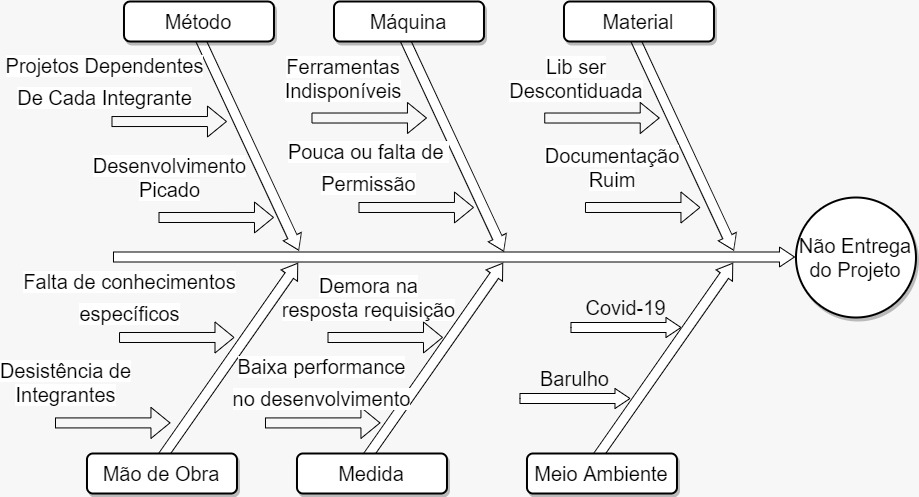
\includegraphics[scale=0.80]{./Figuras/Diagrama causa e efeito.jpeg}
		\end{center}
		\legend{Fonte: os autores (2020)}
	\end{figure}
\end{landscape}

\section{PMBOK}

{É uma metodologia de gerenciamento de projeto internacionalmente reconhecida, essas práticas podem auxiliar na resolução dos recursos humanos, capitais, tecnológicos e técnicos. Além disso, utilizando PMBOK é possível gerir melhor o andamento do projeto e de forma mais coordenada. Segundo \cite{PMG2018} o PMBOK tem conhecimentos já comprovados que são amplamente utilizados, assim como o conhecimento de práticas mais inovadoras e avançadas} Dentre as técnicas de planejamento, pode-se utilizar para estudos e desenvolvimento a EAP -  Estrutura Analítica de Projetos, descrita a seguir.

\subsection{Estrutura Analítica do Projeto}

A Estrutura Analítica do Projeto (EAP) é a divisão estruturada de trabalho do projeto dividido em faixas gerenciadas cuja sua totalidade significa em um entregável ao projeto final.
	
Segundo \cite{PMI2018} o detalhamento da EAP deve chegar até o nível do pacote de trabalho, nível mais baixo na EAP, que é o ponto no qual o custo e o cronograma do trabalho podem ser estimados de forma confiável. Porém o nível de detalhamento desse pacote varia de acordo com a complexidade de cada projeto. \cite{kerzner2017} defende que a EAP deve ser composta por até três níveis, pois se for detalhado com demaseio o custo com o gerenciamento serão também excessivos.

Para o projeto Agil-it foi decidido utilizar 6 faixas de entregáveis:

\begin{subalineas}
	\item {Planejamento};
	\item {Análise};
	\item {Implementação Web};
	\item {Implementação Mobile};
	\item {Testes};
	\item {Implantação}.
\end{subalineas}


\begin{landscape}
	\begin{figure}[htb]
		\caption{\label{EAP}EAP AGIL.IT}
		\begin{center}
			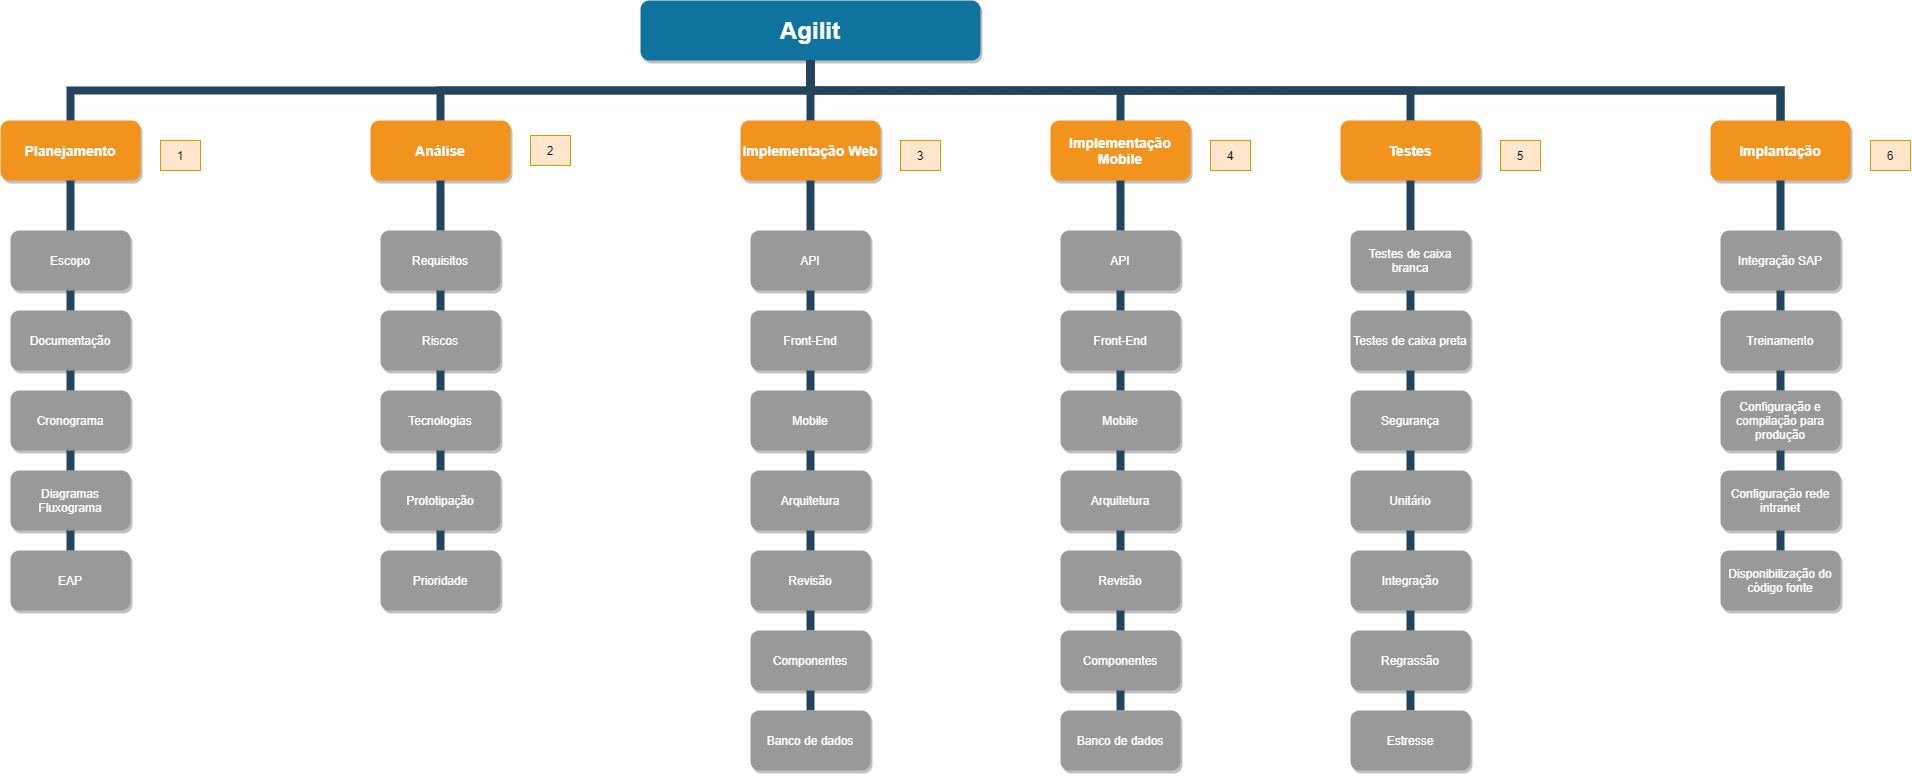
\includegraphics[scale=0.38]{./Figuras/EAP.png}
		\end{center}
		\legend{Fonte: os autores (2020)}
	\end{figure}
\end{landscape}

A figura \ref{EAP} mostra a estrutura e o desenvolvimento que cada faixa requer no projeto. Ela não segue uma ordem cronológica, portanto não é necessário finalizar uma faixa para começar outra, muitas vezes elas são desenvolvidas em conjunto para uma melhor utilização do tempo de projeto.


\subsection{Fluxo de Processos}
% ---

{O fluxo de processo é subdividido em cinco fases principais sobre o fluxo do projeto, iniciação sendo a primeira seguindo de planejamento, execução, monitoramento, controle e finalização. Para \cite{PMG2018} um projeto é desenvolvido a partir de uma ideia, em seguida parte para um plano e após isso é executado e concluído.}

Para a definição dos processos, foi utilizado os seguintes recursos:

\begin{figure}[H]
	\caption{\label{Fluxo-Processos}Fluxo e Processos}
	\begin{center}
		\includegraphics[scale=1]{./Figuras/fluxo-processos.png}
	\end{center}
	\legend{Fonte: \cite{PMG2018}}
\end{figure}



A figura abaixo contém todos os fluxos desenhados para o projeto.

\begin{figure}[H]
	\caption{\label{Fluxo-Processos-eap}Fluxo e Processos AGIL.IT}
	\begin{center}
		\includegraphics[scale=0.24]{./Figuras/fluxo-processos-eap.png}
	\end{center}
	\legend{Fonte: os autores (2020)}
\end{figure}



{\textbf{Iniciação} - Esta é a fase inicial do projeto, nela é determinado a necessidade do projeto, com seus objetivos e justificativas, então é realizado os documentos iniciais onde as melhores estratégias são identificadas e selecionadas.}

{\textbf{Planejamento} - Fase onde deve ser detalhado minuciosamente tudo aquilo que será realizado no projeto, desde cronogramas, interdependências entre atividades, alocação dos recursos envolvidos, análise de custos etc. Esta parte é muito importante pois a execução do projeto será em cima destas atividades para que sejam executadas sem dificuldades e imprevistos.}

{\textbf{Execução} - Nesta fase tudo é onde tudo que foi planejado anteriormente se torne realidade, tendo que ser executado e realizado conforme planejado, qualquer erro cometidas nas fases anteriores fica evidente durante essa fase. }

{\textbf{Monitoramento e Controle} - Esta fase acontece paralelamente às demais fases do projeto, acompanhando e controlando aquilo que está sendo realizado no projeto como um todo, podendo propor ações corretivas e preventivas no menor espaço de tempo possível após a detecção de erros.}


\section{Protótipo}

A prototipação é uma etapa de suma importância no desenvolvimento de projeto de software. Além de melhorar a produtividade da equipe, ela facilita o entendimento dos requisitos do sistema e permite a apresentação de de conceitos e funcionalidades da aplicação de modo simplificado.
Nesse trabalho foi utilizado a prototipação visual cujo ênfase se aplica a estética e usabilidade. Nesse tipo de protótipo é possível identificar o layout e a identidade visual da aplicação. \cite{dextra2013prototipacao}

{Protótipos podem ser gerados de acordo com as seguintes categorias \cite{coyette2004sketchixml}: protótipos em baixa fidelidade que focam na interação, em componentes de interface e na estrutura geral do sistema; protótipos em alta fidelidade que produzem uma imagem real do sistema; protótipos executáveis que produzem o código em uma linguagem de programação, focando em navegação, mas sem ainda levar em consideração as regras de negócio. Cada categoria serve para um propósito específico: protótipos em baixa fidelidade são úteis para demonstrar aos usuários quais atividades o sistema atende e as possibilidades de navegação no sistema, assim como para proporcionar uma visão geral do sistema. Protótipos em alta fidelidade são úteis para demonstrar padrões e guias de estilo. Protótipos executáveis são úteis para demonstrar navegação e testar o uso da interface \cite{rosemberg2008prototipaccao}.Seguindo as definições, o projeto desenvolvido utiliza os protótipos de baixa fidelidade}

\section{Aplicação WEB}
A aplicação web tem como foco o gerenciamento de toda a aplicação envolvendo consultas e cadastros gerais do sistema.
Apesar desse foco acentuado à gestão, é possível desempenhar todos os papeis dentro da aplicação web.

\subsection{Cadastro de Usuário}

\begin{figure}[H]
	\caption{\label{web_cad-user}Cadastro de Usuários}
	\begin{center}
		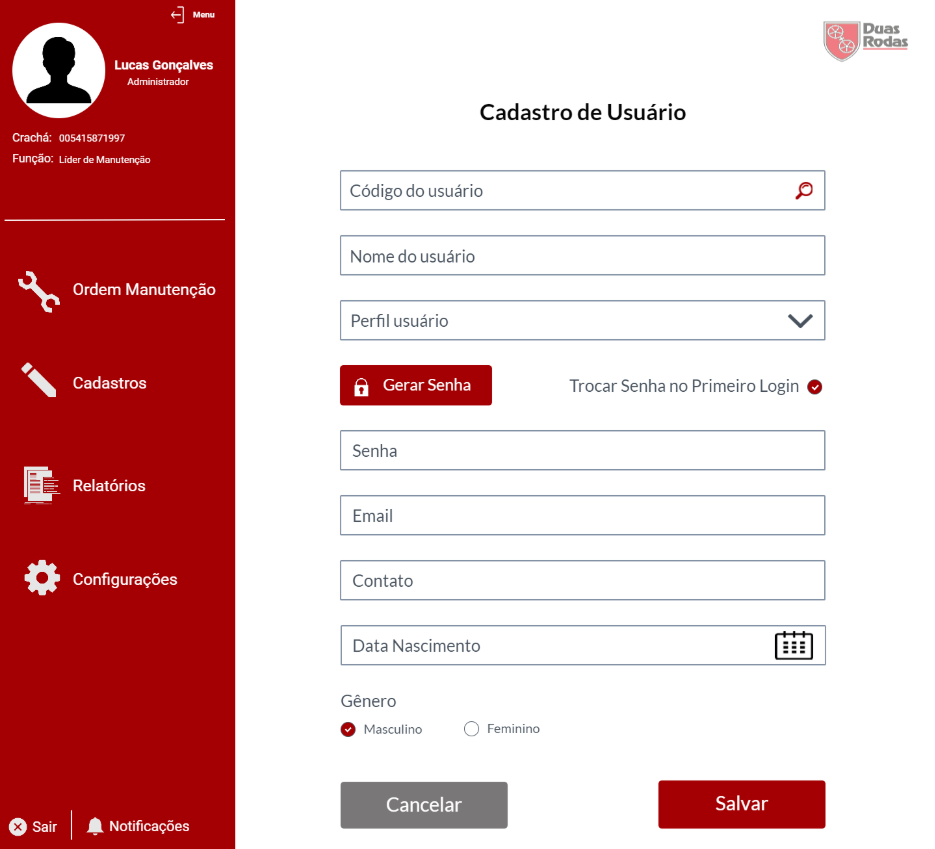
\includegraphics[scale=0.70]{./Figuras/web/cad-user.png}
	\end{center}
	\legend{Fonte: os autores (2020)}
\end{figure}

A tela \ref{web_cad-user} é utilizada para cadastrar usuários no sistema. Caso queira atualizar um registro basta colocar o código dele no primeiro campo ou pesquisar no ícone de lupa. Para cadastrar um novo basta deixar o primeiro campo vazio.

\subsection{Monitor de Ordem de Manutenção: Cards}

\begin{figure}[H]
	\caption{\label{web_monitor-om-card}Monitor de Ordem de Manutenção: Cards}
	\begin{center}
		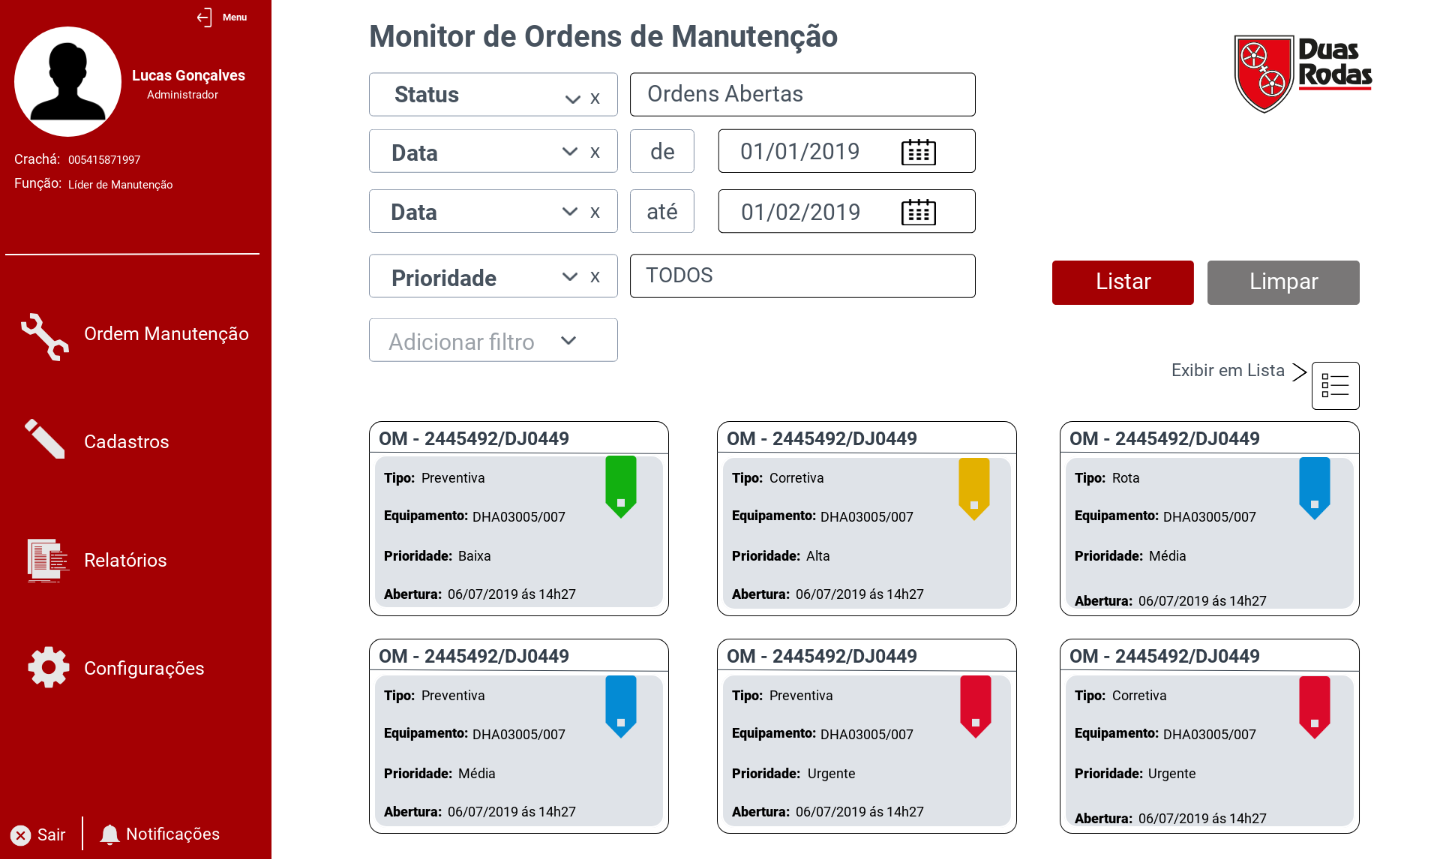
\includegraphics[scale=0.45]{./Figuras/web/monitor-om-card.png}
	\end{center}
	\legend{Fonte: os autores (2020)}
\end{figure}

A tela \ref{web_monitor-om-card} permite a consulta rápida e dinâmica das ordens de manutenção. Nela você pode aplicar os filtros de acordo com as necessidades e será listada em forma de cartões, eles darão acesso à uma tela de detalhamento de ordem de manutenção.

\subsection{Checklist de Segurança}

\begin{figure}[H]
	\caption{\label{web_check-list}Checklist de Segurança}
	\begin{center}
		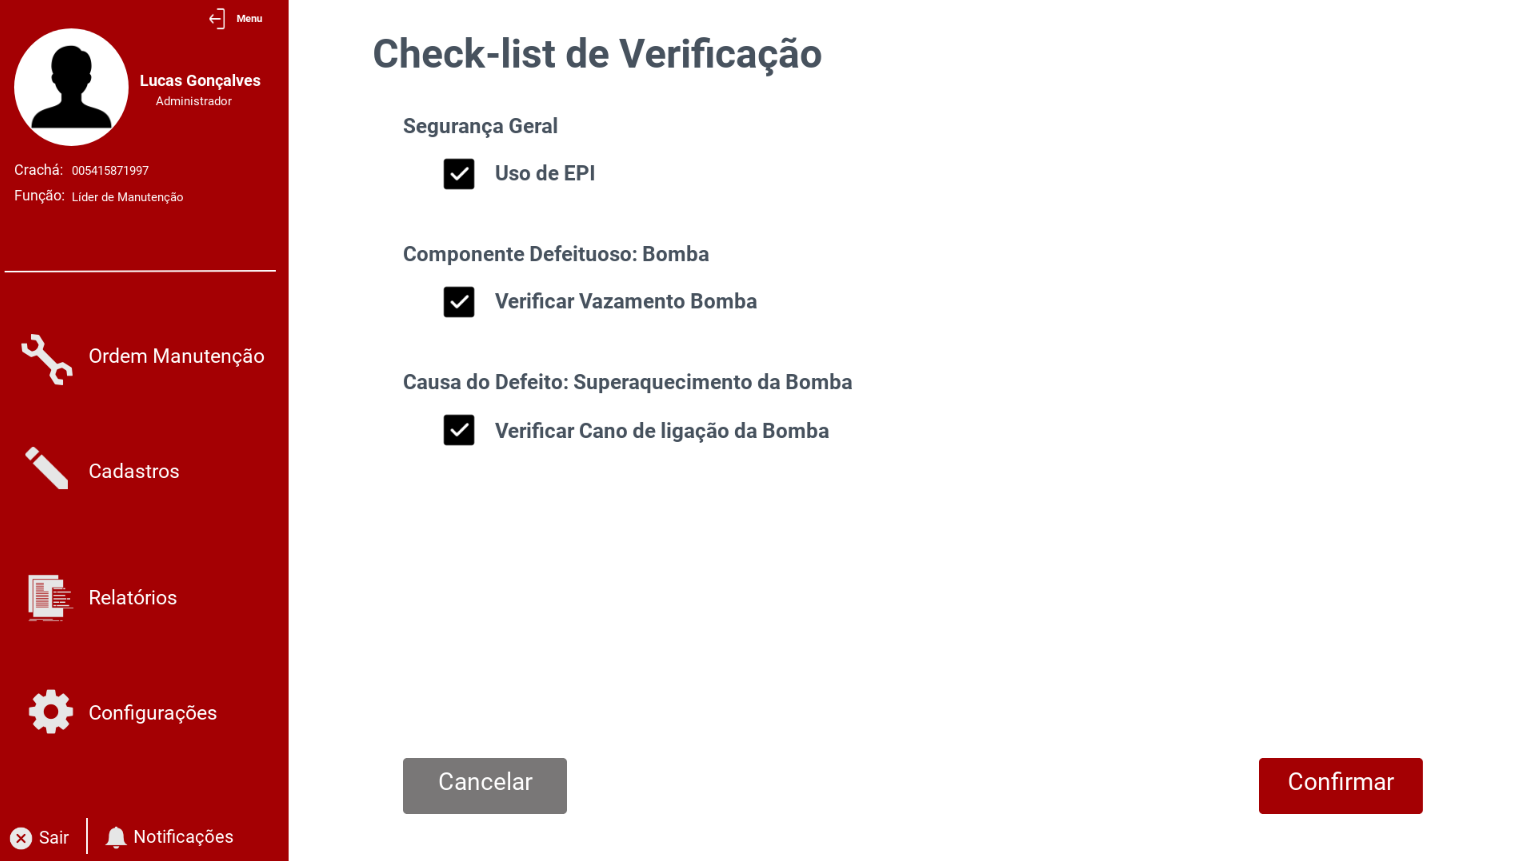
\includegraphics[scale=0.45]{./Figuras/web/check-list.png}
	\end{center}
	\legend{Fonte: os autores (2020)}
\end{figure}

Na tela \ref{web_check-list} o técnico irá marcar a lista de segurança antes de iniciar a ordem de manutenção. Essa listá será gerada dinamicamente de acordo com a parametrização de segurança cadastrado no sistema.

\section{Aplicação Mobile}
A aplicação Mobile é um ponto estratégico do produto, pois sua mobilidade permite com que os técnicos possam atuar na manutenção e realizar anotações e apontamentos no sistema através de um smartphone ou tablet.

\subsection{Monitor}

\begin{figure}[H]
	\caption{\label{mobile_monitor}Monitor}
	\begin{center}
		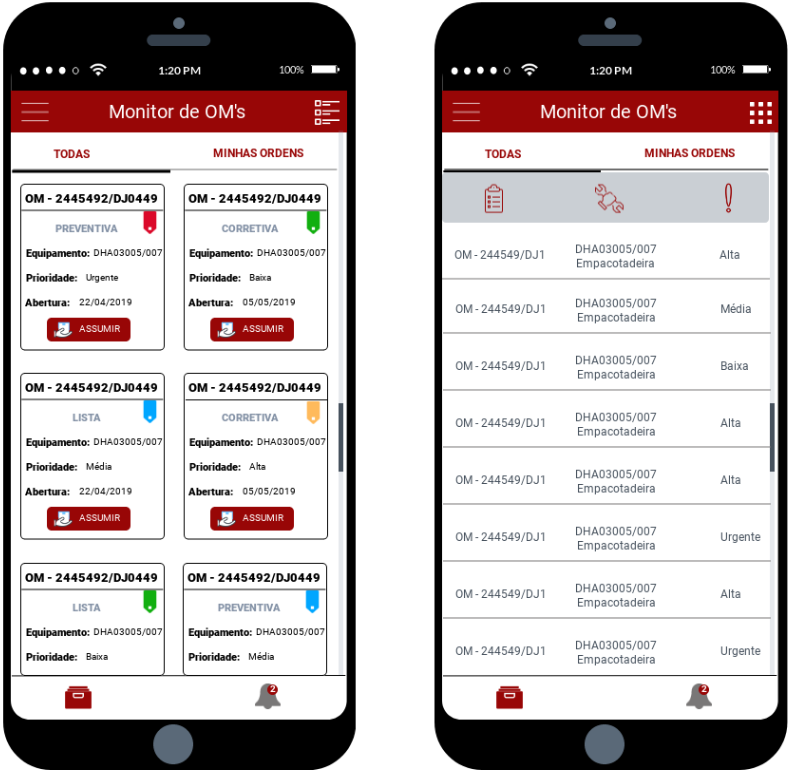
\includegraphics[scale=0.75]{./Figuras/mobile/monitor.png}
	\end{center}
	\legend{Fonte: os autores (2020)}
\end{figure}

Na figura \ref{mobile_monitor} é possível verificar o monitor do técnico de manutenção. Nesse monitor, o técnico consegue rapidamente visualizar as OMs pendentes e seus respectivos status através das bandeiras indicadas no card. As  vermelhas indicam que a OM tem uma prioridade emergente, as amarelas têm prioridade alta, as azuis têm prioridade média e as verdes possuem uma prioridade baixa.

\subsection{Central de Notificações}

\begin{figure}[H]
	\caption{\label{mobile_notificacao}Notificações}
	\begin{center}
		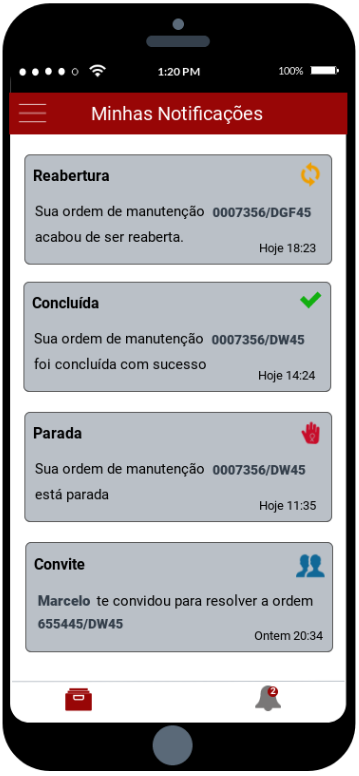
\includegraphics[scale=0.80]{./Figuras/mobile/notificacao.png}
	\end{center}
	\legend{Fonte: os autores (2020)}
\end{figure}

Na tela \ref{mobile_notificacao} é possível verificar notificações do usuário autenticado no sistema.

\subsection{Ordem de Manutenção}

\begin{figure}[H]
	\caption{\label{mobile_om}Ordem de Manutenção}
	\begin{center}
		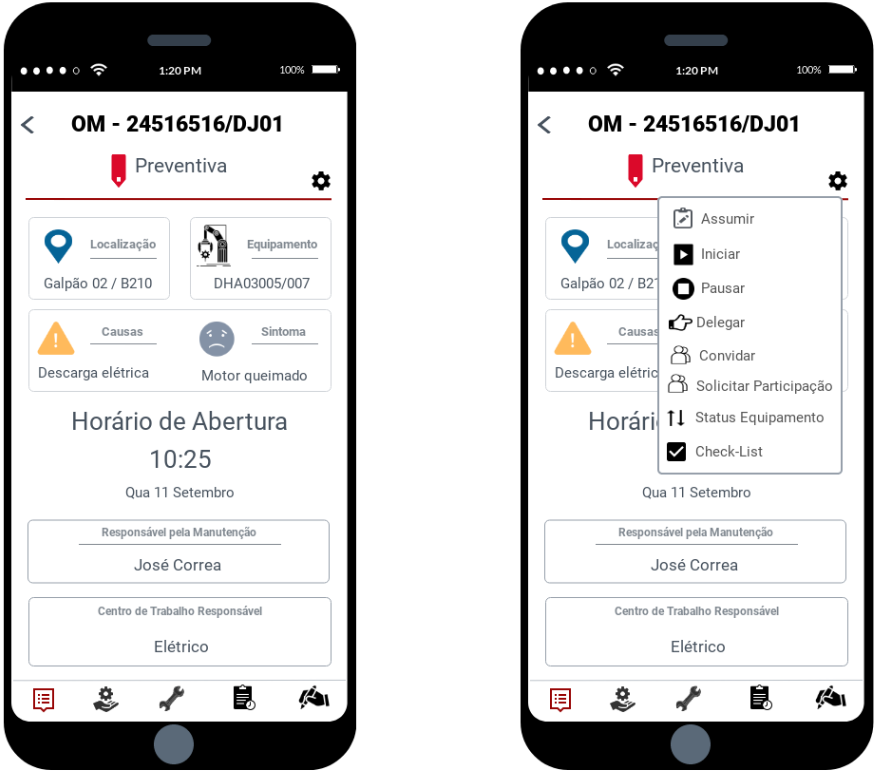
\includegraphics[scale=0.70]{./Figuras/mobile/om.png}
	\end{center}
	\legend{Fonte: os autores (2020)}
\end{figure}

Na tela \ref{mobile_om} será possível acompanhar o andamento de uma ordem de manutenção preventiva e corretiva, ver informações referente à ordem e executar ações nela, como alterar status, adicionar operações e realizar assinaturas.